\documentclass[11pt,a4paper]{article}
\usepackage[utf8]{inputenc}
\usepackage{amsmath}
\usepackage{amsfonts}
\usepackage{amssymb}

\usepackage{natbib}
\usepackage{makecell}
\usepackage{eurosym} 
\usepackage[version=4]{mhchem}
%\usepackage{courier} 
\usepackage[inner=2.5cm,outer=2.5cm]{geometry}

%\usepackage{gensymb}
%\usepackage{subcaption}
%\usepackage{url}
%\usepackage{breakurl}
%\def\UrlBreaks{\do\/\do-}
%
%\usepackage{multibib}
%\newcites{sec}{Bibliography} 
\begin{document}
\title{Mathematical description of the power system model \emph{medea}}
\section{Overview}
\emph{medea} is a simple, stylized and parsimonious power system model.
It simulates investment in intermittent and conventional electricity and heat generation technologies as well as in cross-border electricity transmission capacities.
At the same time, the model determines the system-cost minimizing hourly dispatch of electricity and heat generators to meet price-inelastic demand.
Model results include hourly energy generation by technology and the associated fuel use and CO2 emissions, investment in and decommissioning of conventional and renewable generators and energy storages, hourly cross-border flows of electricity and potentially required transmission capacity expansion, as well as producer and consumer surplus.

A detailed description of the model is provided in the following. Section \ref{sets} gives an overview of the sets and set elements used in \emph{medea}. Sections \ref{parameters} and \ref{variables} introduce the model's parameters and variables, while section \ref{mathmodel} gives a detailed description of the model's mathematical formulation.


% decisions covered - intermittent generation given, thermal and storage dispatch, investment in generation and storage technologies, interconnector capacity
% intermittent technologies: wind onshore \& offshore, pv, run-of-river
% dispatchable technologies: $36$ technologies for dispatchable power and heat generation, including co-generation units for the combined generation of power and heat (for industry or district heating).

%\emph{medea} numerically determines a partial-equilibrium in interconnected electricity markets as would be implemented by a social planner seeking to minimize the total system cost. 
%In particular, this implies that social planners seeking to minimize system cost of individual electricity markets might have an incentive to deviate from the overall cost minimum.
%The model assumes perfectly price inelastic demand for electricity and heat. 
%Within each country we assume sufficient transmission capacities to be in place ('copperplate'). 
%Moreover, heat demand can be met by any heat generator operating in the same country. 

%It covers the hourly dispatch of thermal and hydro storage plants in seven European countries, while taking electricity generation from intermittent sources such as wind or solar energy as given. (Not true because curtailment is possible)
%In addition, the model can determine optimal investment in intermittent and dispatchable generation technologies, storage technologies, and international transmission capacities.

% It can be used to simulate short-term dispatch decisions, but also currently covers 

% determines the system cost-minimizing hourly dispatch of thermal and hydro storage power plants required to meet price-inelastic (residual) demand for electricity and district heat.

% Thermal power plants and hydro storage plants are grouped in $34$ technology clusters. We differentiate the clusters by generation technologies (e.g. steam turbine, combustion turbine, combined cycle, etc.) and by fuels (uranium, lignite, hard coal, natural gas, mineral oil, biomass, water).

% Thermal power plants burn fuels to generate electricity and are constrained in their operation by installed capacities for heat and power generation.

% Heat generation is possible in heat boilers (aggregate capacity $30$ GWth, efficiency $0.9$) or in combined heat and power (CHP) plants, which must respect the limits of their feasible operation region.\footnote{The feasible operation region specifies all viable combinations of heat and power generation along with the required fuel use.}

% Heat generation and consumption are aggregated, i.e. heat generators are not serving specific district heating systems.

% Electricity generation from intermittent renewable sources (wind, solar, run-of-river) is given exogenously but can be curtailed.

% Electricity can also be stored in reservoir and pumped hydro storages.

%Generation from hydro storage plants is constrained by turbine capacity and energy contained in reservoirs of limited size.
%Reservoirs are filled by inflows or by pumping (pumped storages only).
%To better capture operational differences, we model daily, weekly and seasonal reservoir and pumped storage plants separately.
%Electricity exchange with countries outside Austria and Germany is held fixed at hourly quantities realized in 2017.
%To ensure a stable and secure operation of the electricity system, power plants must provide ancillary services such as frequency control or voltage support.
%We assume that this requires generators with an installed capacity of at least $21$ GW \footnote{This is equal to 12.5\% of peak load plus 7.5\% of installed solar and wind power capacity and is broadly in line with findings by \citet{Hirth2015} and \citet{Nicolosi2012}.} to be operational (either generating or pumping in case of pumped hydro storages) at any point in time.
 
%For a mathematical description see \ref{Apndx2}. The model is implemented in GAMS and was solved by Gurobi on an Intel Xeon Gold $6144$ with $264$ GB RAM.
%The model code can be found at \url{https://github.com/sebwehrle/medea}.

\section{Sets} \label{sets}
\begin{tabular}{l l l l}
\textbf{name} & \makecell[l]{\textbf{math} \\ \textbf{symbol}} & \makecell[l]{\textbf{GAMS} \\\textbf{symbol}} & \textbf{elements} \\
\hline \hline
market zones & $z \in Z$ & \texttt{r} & \texttt{AT, DE} \\ \hline

\makecell[l]{time periods \\(hours)} & $t \in T$ & \texttt{t} & \texttt{t1, t2, \ldots, t8760} \\ \hline

\makecell[l]{power generating \\technologies} & $i \in I$ & \texttt{tec} & 

\makecell[l]{ \texttt{nuc, lig\_stm, lig\_stm\_chp,}\\
	\texttt{lig\_boa, lig\_boa\_chp,} \\
	\texttt{coal\_sub, coal\_sub\_chp,} \\
	\texttt{coal\_sc, coal\_sc\_chp,}\\
	\texttt{coal\_usc, coal\_usc\_chp,} \\
	\texttt{coal\_igcc,}\\
	\texttt{ng\_stm, ng\_stm\_chp,} \\
	\texttt{ng\_ctb\_lo, ng\_ctb\_lo\_chp,}\\ 
	\texttt{ng\_ctb\_hi, ng\_ctb\_hi\_chp,}\\
	\texttt{ng\_cc\_lo, ng\_cc\_lo\_chp,}\\
	\texttt{ng\_cc\_hi, ng\_cc\_hi\_chp,}\\
	\texttt{ng\_mtr, ng\_mtr\_chp,} \\
	\texttt{ng\_boiler\_chp,} \\
	\texttt{oil\_stm, oil\_stm\_chp,} \\ 
	\texttt{oil\_ctb, oil\_ctb\_chp,} \\
	\texttt{oil\_cc, oil\_cc\_chp,} \\
	\texttt{bio, bio\_chp,}
	\texttt{heatpump\_pth} 
} \\ \hline

CHP technologies & $j \in I$ & \texttt{tec\_chp} & \makecell[l]{
	\texttt{lig\_stm\_chp, lig\_boa\_chp,}\\
	\texttt{coal\_sub\_chp, coal\_sc\_chp,}\\
	\texttt{coal\_usc\_chp, ng\_stm\_chp,}\\ 
	\texttt{ng\_ctb\_lo\_chp, ng\_ctb\_hi\_chp,}\\
	\texttt{ng\_cc\_lo\_chp, ng\_cc\_hi\_chp,}\\
	\texttt{ng\_mtr\_chp, ng\_boiler\_chp,}\\
	\texttt{oil\_stm\_chp, oil\_ctb\_chp,} \\ 
	\texttt{oil\_cc\_chp, bio\_chp} } \\ \hline

\makecell[l]{power to heat \\ technologies} & $h \in I$ & \texttt{tec\_pth} & \texttt{heatpump\_pth}  \\ \hline

storage technologies & $k \in K$ & \texttt{tec\_strg} & \makecell[l]{
	\texttt{res\_day, res\_week, res\_season,} \\ 
	\texttt{psp\_day, psp\_week, psp\_season,} \\
	\texttt{battery}
	} \\ \hline

\makecell[l]{intermittent \\generators} & $n \in N$ & \texttt{tec\_itm} & \texttt{wind\_on, wind\_off, pv, ror}\\ \hline

fuels & $f \in F$ & \texttt{f} & \makecell[l]{\texttt{nuclear, lignite, coal,} \\ \texttt{gas, oil, biomass, power}} \\ \hline

\makecell[l]{feasible operation \\region limits}& $l \in L$ & \texttt{l} & \texttt{l1, l2, l3, l4} \\ \hline

energy products & $p \in P$ & \texttt{prd} & \texttt{power, heat} \\ \hline \hline
\end{tabular}

\section{Parameters} \label{parameters}
\begin{tabular}{l l l l}
\textbf{name} & \makecell[l]{\textbf{math} \\ \textbf{symbol}} & \makecell[l]{\textbf{GAMS} \\\textbf{symbol}} & \textbf{Unit} \\
\hline \hline
\makecell[l]{minimal conventional \\generation} & $\mu_{z}$ & \texttt{ANCIL\_SERVICE\_LVL(r)} & GW \\ \hline
energy demand & $D_{z,t,p}$ & \texttt{CONSUMPTION(r,t,prd)} & GW \\ \hline
power plant efficiency & $\eta_{i,p,f}$ & \texttt{EFFICIENCY(tec,prd,f)} & $MW / MW_{th}$\\ \hline
fuel emission intensity & $\varepsilon_{f}$ & \texttt{EMISSION\_INTENSITY(f)} & $t \ce{CO2}/MWh_{th}$\\ \hline
\makecell[l]{feasible operating \\region} & $\chi_{i,l,f}$ & \texttt{FEASIBLE\_INPUT(tec,l,f)} & MWh ? \\ \hline
\makecell[l]{feasible operating \\region} & $\psi_{i,l,p}$ & \texttt{FEASIBLE\_OUTPUT(tec,l,prd)} & MWh ? \\ \hline
\makecell[l]{intermittent \\generation profile} & $\phi_{z,t,n}$ & \texttt{GEN\_PROFILE(r,t,tec\_itm)} & \% \\ \hline
%\makecell[l]{exports to not \\modelled regions} & $X$ & \texttt{FLOW\_EXPORTS(r,t)} & GW \\ \hline
%\makecell[l]{imports from not \\modelled regions} & $X$ & \texttt{FLOW\_IMPORTS(r,t)} & GW \\ \hline
\makecell[l]{installed capacity \\of intermittent \\generators} & $r^{0}_{z,n}$ & \texttt{INSTALLED\_CAP\_ITM(r,tec\_itm)} & GW \\ \hline
\makecell[l]{installed capacity \\of thermal generators} & $g^{0}_{z,i}$ & \texttt{INSTALLED\_CAP\_THERM(r,tec)} & GW \\ \hline
\makecell[l]{capital cost of \\intermittent generators \\(specific, annuity)} & $\kappa_{z,n}$ & \texttt{INVESTCOST\_ITM(r,tec\_itm)} & $\frac{mn EUR}{GW}$ \\ \hline
\makecell[l]{capital cost of \\thermal generators \\(specific, annuity)} & $\kappa_{z,i}$ & \texttt{INVESTCOST\_THERMAL(r,tec)} & $\frac{mn EUR}{GW}$ \\ \hline
\makecell[l]{capital cost of \\storages - power \\(specific, annuity)} & $\kappa^{P}_{z,k}$ & \texttt{STORAGE\_PROPERTIES(r,tec\_strg,'cost\_power')} & $\frac{mn EUR}{GW}$ \\ \hline
\makecell[l]{capital cost of \\storages - energy \\(specific, annuity)} & $\kappa^{E}_{z,k}$ & \texttt{STORAGE\_PROPERTIES(r,tec\_strg,'cost\_energy')} & $\frac{mn EUR}{GW}$ \\ \hline
net transfer capacity & $\tau_{z,zz}$ & \texttt{NTC(r,rr)} & GW \\ \hline
\makecell[l]{count of power plants \\of same technology} & $|i_{z}|$ & \texttt{NUM(r,tec)} & . \\ \hline
fixed O\&M cost & $\kappa^o_{i}$ & \texttt{OM\_FIXED\_COST(tec)} & EUR \\ \hline
variable O\&M cost & $\kappa^o_{i}$ & \texttt{OM\_VAR\_COST(tec)} & EUR / MWh \\ \hline
% day-ahead price & $p_{el}$ & \texttt{PRICE\_DA(t,r)} & EUR / MWh \\ \hline
\ce{CO2} price & $p^{e}_{t,z}$ & \texttt{PRICE\_EUA(t,r)} & EUR / t CO2 \\ \hline
fuel price & $p_{t,z,f}$ & \texttt{PRICE\_FUEL(t,r,f)} & EUR / MWh \\ \hline
reservoir inflows & $\rho_{z,t,k}$ & \texttt{RESERVOIR\_INFLOWS(r,t,tec\_strg)} & MW \\ \hline
max power out & $\bar{s}^{out}_{z,k}$ & \texttt{STORAGE\_PROPERTIES(r,tec\_strg,'power\_out')} & GW \\ \hline
max power in & $\bar{s}^{in}_{z,k}$ & \texttt{STORAGE\_PROPERTIES(r,tec\_strg,'power\_in')} & GW \\ \hline
max energy stored & $\bar{v}_{z,k}$ & \texttt{STORAGE\_PROPERTIES(r,tec\_strg,'energy\_max')} & . \\ \hline
efficiency power out & $\eta^{out}_{z,k}$ & \texttt{STORAGE\_PROPERTIES(r,tec\_strg,'efficiency\_out')} & . \\ \hline
efficiency power in & $\eta^{in}_{z,k}$ & \texttt{STORAGE\_PROPERTIES(r,tec\_strg,'efficiency\_in')} & . \\ \hline
\hline
\end{tabular}

\section{Variables} \label{variables}
\begin{tabular}{l l l l}
\textbf{name} & \makecell[l]{\textbf{math} \\ \textbf{symbol}} & \makecell[l]{\textbf{GAMS} \\\textbf{symbol}} & \textbf{Unit} \\
\hline \hline
%cost variables
system cost & $C_{z}$ & \texttt{cost(r)} & EUR \\ \hline
emission cost & $C^{e}_{z,t,i}$ & \texttt{cost\_emission(r,t,tec)} & EUR \\ \hline
fuel cost & $C^{f}_{z,t,i}$ & \texttt{cost\_fuel(r,t,tec)} & EUR \\ \hline
total o\&m cost & $C^{om}_{z,i}$ & \texttt{cost\_om(r,tec)} & EUR \\ \hline
\makecell[l]{capital cost of \\generators} & $C_{z}^{inv,i}$ & \texttt{cost\_invgen(r)} & EUR \\ \hline
\makecell[l]{capital cost of \\storages} & $C_{z}^{inv,k}$ & \texttt{cost\_invstrg(r)} & EUR \\ \hline
\makecell[l]{capital cost of \\interconnectors} & $C_{z}^{inv,ic}$ & \texttt{cost\_gridexpansion(r)} & EUR \\ \hline
% investment and decommissioning variables
\makecell[l]{added capacity of \\intermittents} & $r^{+}_{z,n}$ & \texttt{invest\_res(r,tec\_itm)} & GW \\ \hline
\makecell[l]{added capacity of \\conventionals} & $g^{+}_{z,i}$ & \texttt{invest\_thermal(r,tec)} & GW \\ \hline
\makecell[l]{added storage \\capacity (power)} & $v^{+}_{z,k}$ & \texttt{invest\_storage\_power(r,tec\_strg)} & EUR \\ \hline
\makecell[l]{added in storage \\capacity (energy)} & $s^{+}_{z,k}$ & \texttt{invest\_storage\_energy(r,tec\_strg)} & EUR \\ \hline
\makecell[l]{added transmission \\capacity} & $x^{+}_{z,zz}$ & \texttt{invest\_ntc(r,rr)} & EUR \\ \hline
\makecell[l]{decommissioned \\capacity of \\conventionals} & $g^{-}_{z,i}$ & \texttt{decommission(r,tec)} & GW \\ \hline
% dispatch variables
\makecell[l]{energy generated by \\conventionals} & $g_{z,t,i,p}$ & \texttt{q\_gen(r,t,tec,prd)} & GW \\ \hline
\makecell[l]{electricity generated \\by intermittents} & $r_{z,t,n}$ & \texttt{q\_itm(r,t,tec\_itm)} & GW \\ \hline
\makecell[l]{operating region \\weight} & $w_{z,t,i,l}$ & \texttt{cc\_weights(r,t,tec,l)} & . \\ \hline
\makecell[l]{fuel burn for energy \\generation} & $b_{z,t,i,f}$ & \texttt{q\_fueluse(r,t,tec,f)} & GW \\ \hline
energy stored in & $s^{in}_{z,t,k}$ & \texttt{q\_store\_in(r,t,tec\_strg)} & GW \\ \hline
energy stored out & $s^{out}_{z,t,k}$ & \texttt{q\_store\_out(r,t,tec\_strg)} & GW \\ \hline
\makecell[l]{storage energy \\content} & $v_{z,t,k}$ & \texttt{storage\_level(r,t,tec\_strg)} & GWh \\ \hline
\makecell[l]{electricity net \\export} & $x_{z,zz,t}$ & \texttt{flow(r,rr,t)} & GW \\ \hline
curtailed energy & $\Omega^{-}_{z,t,p}$ & \texttt{q\_curtail(r,t,prd)} & GW \\ \hline
non-served energy & $\Omega^{+}_{z,t,p}$ & \texttt{q\_nonserved(r,t,prd)} & GW \\ \hline
% other variables
\ce{CO2} emissions & $e_{z}$ & \texttt{emissions(r)} & t \ce{CO2} \\ \hline

\end{tabular}

\newpage
\section{Mathematical description} \label{mathmodel}
Objective function: total system cost, minimization
\begin{align}
\min C = \sum_{z} (C_{z})
\end{align}
System cost consist of fuel cost $C^{f}_{z,t,i}$, emission cost $C^{e}_{z,t,i}$, operation and maintenance cost $C^{om}_{z,i}$, and capital costs of investment in generation, storage and transmission equipment plus the cost of non-served load that accrues when demand is not met, i.e. when there is a black out.
\begin{align}
\begin{split}
C_{z} = \sum_{t,i} & C^{f}_{z,t,i} + \sum_{t,i} C^{e}_{z,t,i} + \sum_{i} C^{om}_{z,i} + C^{inv,i}_{z} + \\
& C^{inv,n}_{z} + C^{inv,k}_{z} + C^{inv,ic}_{z} + \sum_{t,p} C^{nse}_{z,t,p} \qquad \qquad \forall z
\end{split}
\end{align}


Our power system model uses a linear programming formulation of the economic dispatch problem for thermal units within the Austro-German bidding zone. Operation of pumped storage plants is also formulated as a linear problem.
The model's objective is to minimize total system cost, the sum of fuel, emission and operation and maintenance cost along with the cost associated with curtailment of renewable energies and loss of load.
\begin{align}
\min \left(\sum_{t,g,f}\left(\left(P_{t,f} + em_{f} P_{t,eua}+om_{g}\right) qf_{t,g,f} + qns_{t,p} M + qct_{t} N \right) \right)
\end{align}
In each hour the market has to clear, such that electricity supply from thermal and net generation from hydro storage plants plus power generation from non-dispatchable sources (wind energy, photovoltaics, and run-of-river hydro plants) equals electricity demand less net imports of electricity.
\begin{align}\label{12}
\begin{split}
D_{t,pwr} - Q_{t,nip} = \sum_{g} \left(q p_{t,g,pwr} \right) + \sum_{g\in PSP} \left(qpsp_{t,g} - ppsp_{t,g} \right) \\
+ Q_{t,we} + Q_{t,pv} + Q_{t,ror}, \forall t
\end{split}
\end{align}
In linear (economic dispatch) models, the marginals ('shadow prices') on equation (\ref{12}) can be interpreted as power prices in an energy-only market. We use these marginals to derive the pass-through from emission prices to power prices.
As we also consider co-generation of heat and power in our model, we introduce the heat balance equation (\ref{13}). Heat supply from CHP units and heat boilers must be adequate to meet district heating demand $D_{t,ht}$.
\begin{align}\label{13}
D_{t,ht} \leq \sum_{g \in CHP} \left( qp_{t,g,ht} \right) + qns_{t,p}, \forall t
\end{align}
Hourly generation of power and heat is constrained by installed capacity. 
\begin{align}
qp_{t,g,p} \leq \bar{C}_{g,p}, \forall t
\end{align}
Coproduction of heat and power in CHP-plants is governed by
\begin{align}
\sum_{l} sconv_{t,g,l} = 1, \forall g \in CHP \\
\sum_{l} sconv_{t,g,l} ORP_{g,l,p} = qp_{t,g,p}, \forall g \in CHP \\
\sum_{l} sconv_{t,g,l} ORF_{g,l,f} \leq qfuel_{t,g,f}
\end{align}
Power production by power-only generators is modelled as a linear function of plant efficiency
\begin{align}
qp_{t,g,pwr} \leq \sum_{f} \eta_{g,f,pwr} qf_{t,g,f}, \forall t, g \notin CHP  
\end{align}
Ancillary services must be provided by operating thermal generation units or active hydro storage plants (regardless of whether they are pumping or turbining).
\begin{align}
\underline{a} \leq qp_{t,g,pwr} + qpsp_{h,g} + qstor_{t,g}, \forall t
\end{align}
Operation of pumped storage plants is subject to the equations
\begin{align}
qpsp_{h,g} \eta_{g} \leq \overline{C}_{g}, \forall t, g \in PSP \\
ppsp_{t,g} \leq \overline{C}_{g}, \forall t, g \in PSP \\
qstor_{t,g} - qstor_{t-1, g} = ppsp_{h,g} \eta_{g} - qpsp_{h,g} \\
qstor_{t,g} \leq \overline{STOR}_{g}, \forall t, g \in PSP
\end{align}

\section{Data}
Information regarding the power plant stock (generation capacities, technology, locations) in Germany are based on data provided by the Open Power System Data (OPSD) project \citep{OPSD2018a}.
Data on Austrian power plants was collected through own research and includes information from the regulatory body~\citep{EControl2003}, sector associations~\citep{OeEn2017}, operating companies, and water registers of federal authorities~\citep{LandVorarlberg2018, LandTirol2018}.
Hourly electricity generation from intermittent sources (solar PV, wind) and load in Austria and Germany is also sourced from \citet{OPSD2018b}. 
Further time series on international commercial electricity exchanges, the aggregate filling rate of hydro reservoirs and storage plants, and the actual electricity generation and consumption of hydro power plants (including run-of-river plants) are obtained from ENTSO-E's transparency platform~\citep{ENTSOE2018}.
We approximate inflows of water to reservoirs in Austria by combining downsampled data on weekly water reservoir levels with hourly electricity generation and pumping from hydro reservoirs and pumped storage plants.\footnote{In Germany, 98\% of the installed hydro storage capacity is pumped hydro power so that we abstract from inflows to German hydro storage plants.}
Hourly district heating demand is estimated based on synthetic load profiles for natural gas demand~\citep{Almbauer2009}.
These load profile make use of daily average temperatures from MERRA-2 satellite data~\citep{GMAO2015} and are scaled to total final consumption of district heat in Germany and Austria.\footnote{As final data for the consumption of district heat in 2017 was not published at the time of writing, we scale 2016 district heat consumption by the relative change in heating degree days from 2016 to 2017~\citep{AGEB2018a, OeStat2018}.}
Realized prices of hard coal, natural gas and EU emission allowances for the year 2017 are taken from the \citet{EEX2019}.
Prices for mineral oil are approximated on the basis of prices for Brent crude oil as published by the~\citet{EIA2018}.
As there are no market prices for nuclear fuel and lignite, we estimate lignite cost at $5.50$~\euro{}/MWh (including mining, but excluding emission cost) and $3.50$~\euro{}/MWh for nuclear fuel.
Descriptive Statistics for all used time series are displayed in Table~\ref{Tab2}.

\begin{table}[t!]
\caption{Descriptive statistics}
\smallskip
\centering
\begin{tabular}{c c c c c c c}
\hline
 & Unit & Min & Max & Mean & Std. Dev & Source \\ \hline \hline
Wind & $GW$ & $0.279$ & $41.72$ & $12.49$ & $9.03$ & OPSD \\ \hline
Solar PV & $GW$ & $0$ & $28.33$ & $4.23$ & $6.49$ & OPSD \\ \hline
Run-of-river & $GW$ & $2.08$ & $7.13$ & $4.78$ & $1.13$ & ENTSO-E \\ \hline
\makecell{Reservoir \\ inflows} & $GW$ & $0$ & $2.14$ & $0.79$ & $0.59$ & \makecell{own\\ calculations} \\ \hline
\makecell{Electricity \\consumption} & $GW$ & $38.52$ & $96.77$ & $69.09$ & $12.59$ & ENTSO-E \\ \hline
\makecell{District heat \\ consumption} & $GW$ & $1.54$ & $42.04$ & $13.49$ & $9.60$ & \makecell{own \\calculations} \\ \hline
\makecell{Net imports \\ (commercial \\exchange)} & $GW$ & $-13.74$ & $7.07$ & $-4.87$ & $2.93$ & ENTSO-E\\ \hline
\makecell{Coal price \\(API2)} & \euro{}$/MWh_{th}$ & $8.32$ & $11.36$ & $9.65$ & $0.72$ & eex \\ \hline
\makecell{Natural gas \\price (NCG)} & \euro{}$/MWh_{th}$ & $15.91$ & $19.02$ & $17.27$ & $0.87$ & eex\\ \hline
\makecell{Mineral oil \\price} & \euro{}$/MWh_{th}$ & $23.18$ & $32.93$ & $28.25$ & $2.57$ & EIA\\ \hline
\makecell{EU Emission \\Allowance price} & \euro{}$/MWh_{th}$ & $4.41$ & $8.21$ & $5.89$ & $1.11$ & eex\\
\hline \hline
\end{tabular}
\label{Tab2}
\end{table}

%\section{Model calibration and goodness-of-fit}
%\begin{figure}[t]
%\centering
%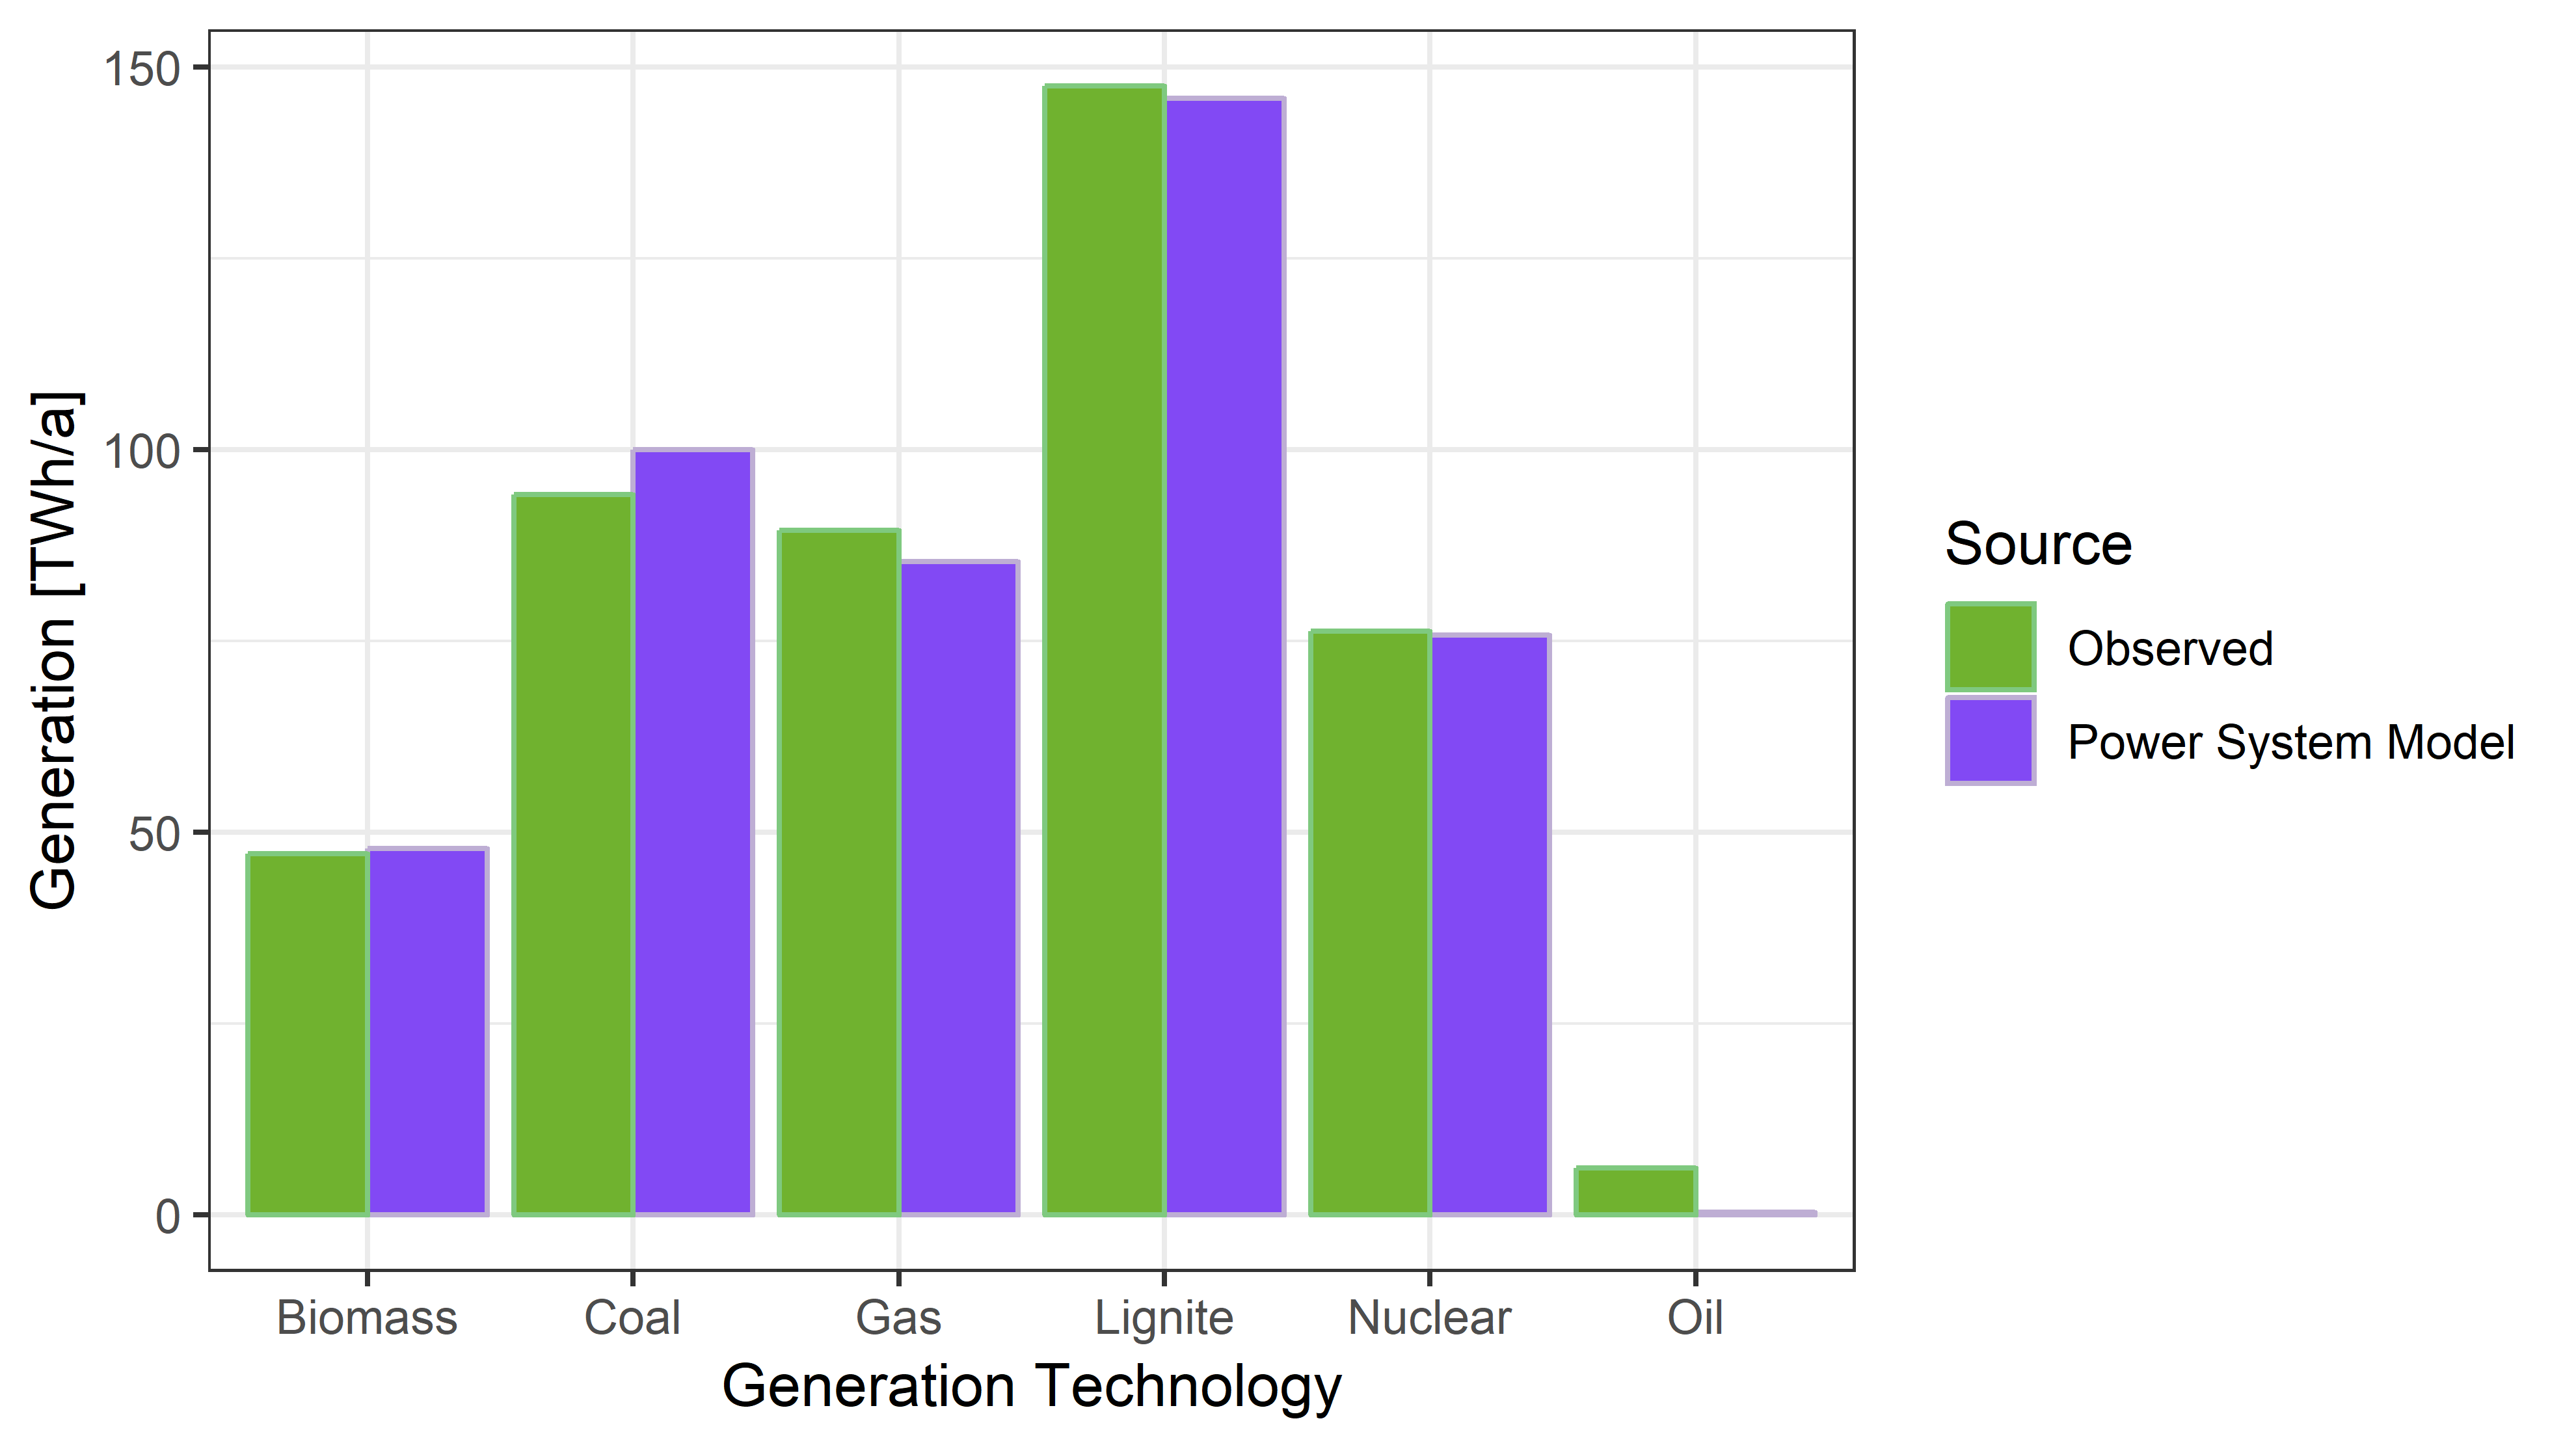
\includegraphics[scale=0.75]{Figure2_calibration.png}
%\caption{Actual and model derived fuel burn (2017)}\label{Fig2}
%\end{figure}
%
%We use power plant efficiencies and availabilities to calibrate our power system model on actual data for quantities of fuel burnt for power generation~\citep{AGEB2018, OeStat2018} and greenhouse gas emissions \citep{UBA_DE2018a, UBA_DE2018b} from 2017.
%\footnote{For Austria, the most recent data on GHG emissions and fuel burn for power generation available at the time of writing relates to 2016. As Austria’s electricity consumption is only around one tenth of Germany’s and roughly two-third of power generation in Austria stems from hydro power plants, the induced error should, however, be small.} 
%
%As visible in figure \ref{Fig2}, our model is able to replicate fuel burn and emissions fairly well, although the use of coal is somewhat overstated ($+5.9$ TWh), while consumption of natural gas and oil are underestimated by $4.0$ TWh and $5.7$ TWh. Overall, modelled \ce{CO2} emissions from power generation of $316.4$ million tonnes are falling short of near time estimates by around $2.4\%$ or $7.9$ million tonnes.
%Comparing the model-derived hourly shadow prices of electricity to actual day-ahead prices at the European Energy Exchange in 2017, we observe a correlation of $0.80$ and a root mean squared error (RMSE) of $10.91$.
\end{document}